% ============================================================
%  M.Tech Thesis  —  NIT Rourkela
%  Author : Abhishek Kumar Singh (224CS1022)
%  Supervisor : Prof. Bibhudatta Sahoo
% ============================================================
\documentclass[12pt,a4paper,oneside]{report}

% ── Packages ─────────────────────────────────────────────
\usepackage[a4paper,
            left=1.5in, right=1.0in,
            top=1.0in,  bottom=1.0in]{geometry}
\usepackage{setspace}
\usepackage{fontenc}
\usepackage{inputenc}
\usepackage{times}
\usepackage{graphicx}
\usepackage{booktabs}
\usepackage{tabularx}
\usepackage{longtable}
\usepackage{multirow}
\usepackage{amsmath,amssymb,amsfonts}
\usepackage{algorithm}
\usepackage{algpseudocode}
\usepackage{hyperref}
\usepackage{url}
\usepackage{cite}

\usepackage{caption}
\usepackage{subcaption}
\usepackage{fancyhdr}
\usepackage{titlesec}
\usepackage{tocloft}
\usepackage{emptypage}
\usepackage{xcolor}
\usepackage{float}
\usepackage{microtype}
\usepackage{pgfplots}
\pgfplotsset{compat=1.18}
\usepackage{tikz}

% ── Hyperref setup ───────────────────────────────────────
\hypersetup{
    colorlinks = true,
    linkcolor  = black,
    citecolor  = black,
    urlcolor   = blue,
    pdftitle   = {DRL-LSTM-LBRO: Adaptive Load Balancing in IoT Edge Computing},
    pdfauthor  = {Abhishek Kumar Singh},
}

% ── Line spacing ─────────────────────────────────────────
\onehalfspacing

% ── Chapter / section title formatting ───────────────────
\titleformat{\chapter}[display]
  {\normalfont\large\bfseries\centering}
  {CHAPTER \thechapter}{0pt}{\large\bfseries\MakeUppercase}
\titlespacing*{\chapter}{0pt}{-20pt}{20pt}

\titleformat{\section}{\normalfont\normalsize\bfseries\raggedright}{\thesection}{1em}{}
\titleformat{\subsection}{\normalfont\normalsize\bfseries\raggedright}{\thesubsection}{1em}{}

% ── Header / footer ──────────────────────────────────────
\pagestyle{fancy}
\fancyhf{}
\fancyhead[R]{\small\leftmark}
\fancyfoot[C]{\thepage}
\renewcommand{\headrulewidth}{0.4pt}

% ── Paragraph style ──────────────────────────────────────
\setlength{\parindent}{0.5in}
\setlength{\parskip}{0pt}

% ── ToC / LoF / LoT formatting ───────────────────────────
\renewcommand{\cftchapfont}{\bfseries}
\renewcommand{\cftchappagefont}{\bfseries}
\setlength{\cftbeforechapskip}{6pt}

% ─────────────────────────────────────────────────────────
\begin{document}

% ── Front matter (Roman numerals) ────────────────────────
\pagenumbering{roman}

% ── Title Page ───────────────────────────────────────────
\begin{titlepage}
\begin{center}

\vspace*{0.5cm}
{\Large\bfseries
DRL-LSTM-LBRO: Adaptive Load Balancing in IoT\\[4pt]
Edge Computing via Deep Reinforcement Learning\\[4pt]
with LSTM-Augmented State Prediction
}

\vspace{1.0cm}
{\normalsize A thesis submitted in partial fulfillment of the requirements\\
for the degree of}

\vspace{0.5cm}
{\large\bfseries Master of Technology}\\[4pt]
{\normalsize in}\\[4pt]
{\large\bfseries Computer Science and Engineering}

\vspace{0.8cm}
{\normalsize by}

\vspace{0.5cm}
{\large\bfseries Abhishek Kumar Singh}\\[4pt]
{\normalsize (Roll No. 224CS1022)}

\vspace{1.2cm}
\includegraphics[width=2.5cm]{frontmatter/nitr_logo.png}

\vspace{0.8cm}
{\large\bfseries Department of Computer Science and Engineering}\\[4pt]
{\large\bfseries National Institute of Technology Rourkela}\\[4pt]
{\normalsize Rourkela -- 769008, Odisha, India}

\vspace{0.8cm}
{\normalsize May 2026}

\end{center}
\end{titlepage}

% ── Supervisor's Certificate ─────────────────────────────
\chapter*{Certificate}
\addcontentsline{toc}{chapter}{Certificate}
\thispagestyle{plain}

\begin{center}
{\large\bfseries National Institute of Technology Rourkela}\\[6pt]
{\normalsize Rourkela -- 769008, Odisha, India}
\end{center}

\vspace{1.5cm}

This is to certify that the thesis entitled \textbf{``DRL-LSTM-LBRO:
Adaptive Load Balancing in IoT Edge Computing via Deep Reinforcement
Learning with LSTM-Augmented State Prediction''} submitted by
\textbf{Abhishek Kumar Singh} (Roll No.\ 224CS1022) in partial
fulfillment of the requirements for the award of the degree of
\textbf{Master of Technology} in \textbf{Computer Science and
Engineering} at the \textbf{National Institute of Technology Rourkela}
is an authentic work carried out by him under my supervision and
guidance.

To the best of my knowledge, the matter embodied in the thesis has
not been submitted to any other university or institution for the
award of any degree or diploma.

\vspace{3.0cm}

\noindent
\begin{minipage}[t]{0.55\textwidth}
\end{minipage}
\hfill
\begin{minipage}[t]{0.40\textwidth}
\textbf{Prof.\ Bibhudatta Sahoo}\\
Department of Computer Science\\
and Engineering\\
National Institute of Technology\\
Rourkela -- 769008, India\\[6pt]
Date: \underline{\hspace{3cm}}
\end{minipage}

% ── Declaration ──────────────────────────────────────────
\chapter*{Declaration}
\addcontentsline{toc}{chapter}{Declaration}
\thispagestyle{plain}

I, \textbf{Abhishek Kumar Singh}, Roll No.\ \textbf{224CS1022},
hereby declare that the thesis titled \textbf{``DRL-LSTM-LBRO:
Adaptive Load Balancing in IoT Edge Computing via Deep Reinforcement
Learning with LSTM-Augmented State Prediction''} submitted to the
\textbf{Department of Computer Science and Engineering, National
Institute of Technology Rourkela}, for the award of the degree of
\textbf{Master of Technology}, is a record of original research work
carried out by me under the supervision of
\textbf{Prof.\ Bibhudatta Sahoo}.

I further declare that the work reported in this thesis has not been
submitted, either in part or in full, to any other university or
institution for the award of any degree or diploma. Wherever
contributions from other published works have been incorporated, due
acknowledgement has been made and references have been cited
appropriately.

\vspace{3.0cm}

\noindent
\begin{minipage}[t]{0.55\textwidth}
Place: Rourkela\\
Date: \underline{\hspace{3cm}}
\end{minipage}
\hfill
\begin{minipage}[t]{0.40\textwidth}
\textbf{Abhishek Kumar Singh}\\
Roll No.\ 224CS1022\\
M.Tech (CSE)\\
NIT Rourkela
\end{minipage}

% ── Acknowledgement ──────────────────────────────────────
\chapter*{Acknowledgement}
\addcontentsline{toc}{chapter}{Acknowledgement}
\thispagestyle{plain}

% TODO: Fill in your personal acknowledgement here.
% Below is a structural placeholder — rewrite in your own words.

Completing this thesis has been a journey that would not have been
possible without the support and encouragement of several people, and
I take this opportunity to express my sincere gratitude to each of
them.

First and foremost, I am deeply indebted to my supervisor,
\textbf{Prof.\ Bibhudatta Sahoo}, Department of Computer Science and
Engineering, NIT Rourkela, for his invaluable guidance, patience, and
constant motivation throughout this work. His insightful suggestions
and constructive criticism shaped both the direction and quality of
this research.

I extend my thanks to the faculty members and staff of the Department
of Computer Science and Engineering for creating an environment
conducive to research. I am also grateful to my fellow research
scholars and classmates for many stimulating discussions and for making
my time at NIT Rourkela memorable.

I owe a great deal to my parents and family, whose unwavering belief
in me has been a source of strength at every step. This work is as
much theirs as it is mine.

\vspace{1.5cm}
\noindent
\begin{flushright}
\textbf{Abhishek Kumar Singh}\\
224CS1022\\
Department of CSE, NIT Rourkela
\end{flushright}

% ── Abstract ─────────────────────────────────────────────
\chapter*{Abstract}
\addcontentsline{toc}{chapter}{Abstract}
\thispagestyle{plain}

The rapid proliferation of Internet of Things (IoT) devices has placed
growing pressure on mobile edge computing (MEC) infrastructure, where
edge cloudlets must handle large volumes of latency-sensitive tasks
under tight resource constraints. Conventional load balancing methods
that rely on fixed rules or purely reactive heuristics tend to
struggle in such settings because they neither anticipate future
congestion nor adapt their policies based on past experience.

This thesis presents \textbf{DRL-LSTM-LBRO}, a two-stage intelligent
task scheduling framework that addresses these limitations by combining
short-horizon load forecasting with deep reinforcement learning-based
placement decisions. In the first stage, a per-cloudlet GRU-LSTM
predictor estimates near-future CPU and RAM utilisation from a sliding
window of historical observations. These predictions are incorporated
into the state representation seen by a Double Deep Q-Network (DDQN)
agent, which learns a task placement policy through interaction with a
simulated MEC environment modelled as an M/M/$c$ queuing system. The
reward function jointly penalises task drops, deadline violations,
end-to-end latency, energy consumption, and load imbalance, preventing
the well-known policy-collapse behaviour where an agent routes all
traffic to the most capable node.

Simulation-based evaluation on a three-cloudlet topology using task
workloads derived from the Google Borg cluster trace shows that
DRL-LSTM-LBRO achieves a \textbf{0.58\%} average task drop rate and
\textbf{0.260~s} average end-to-end latency over 500 evaluation
episodes (ten random seeds). Compared to five published load balancing
algorithms and a Proximal Policy Optimisation (PPO) baseline, the
proposed framework reduces drop rates by up to 88.9\% and latency by
up to 26.3\%. A scalability experiment extending the topology to six
cloudlets confirms that the framework generalises without architectural
modifications, achieving a 37.4\% drop reduction over the classical
LBRO baseline.

\vspace{0.5cm}
\noindent\textbf{Keywords:} Mobile edge computing, load balancing,
deep reinforcement learning, Double DQN, LSTM, IoT task scheduling,
M/M/$c$ queuing, scalability.


\tableofcontents
\clearpage

\listoffigures
\addcontentsline{toc}{chapter}{List of Figures}
\clearpage

\listoftables
\addcontentsline{toc}{chapter}{List of Tables}
\clearpage

% ── List of Abbreviations ────────────────────────────────
\chapter*{List of Abbreviations}
\addcontentsline{toc}{chapter}{List of Abbreviations}

\begin{tabular}{ll}
\textbf{5G}       & Fifth Generation Wireless Network \\
\textbf{API}      & Application Programming Interface \\
\textbf{CPU}      & Central Processing Unit \\
\textbf{CRI}      & Composite Resource Index \\
\textbf{DDQN}     & Double Deep Q-Network \\
\textbf{DQN}      & Deep Q-Network \\
\textbf{DRL}      & Deep Reinforcement Learning \\
\textbf{EMA}      & Exponential Moving Average \\
\textbf{GAE}      & Generalised Advantage Estimation \\
\textbf{GB}       & Gigabyte \\
\textbf{GRU}      & Gated Recurrent Unit \\
\textbf{IoT}      & Internet of Things \\
\textbf{JFI}      & Jain's Fairness Index \\
\textbf{LAN}      & Local Area Network \\
\textbf{LBRO}     & Load Balancing based on Resource Occupancy \\
\textbf{LC}       & Least Connection \\
\textbf{LSTM}     & Long Short-Term Memory \\
\textbf{LTS}      & Long Term Support \\
\textbf{MB}       & Megabyte \\
\textbf{Mbps}     & Megabits Per Second \\
\textbf{MDP}      & Markov Decision Process \\
\textbf{MEC}      & Mobile Edge Computing \\
\textbf{MIPS}     & Million Instructions Per Second \\
\textbf{ML}       & Machine Learning \\
\textbf{NFV}      & Network Function Virtualisation \\
\textbf{OS}       & Operating System \\
\textbf{PPO}      & Proximal Policy Optimisation \\
\textbf{QoS}      & Quality of Service \\
\textbf{RAM}      & Random Access Memory \\
\textbf{RF}       & Random Forest \\
\textbf{RL}       & Reinforcement Learning \\
\textbf{RNN}      & Recurrent Neural Network \\
\textbf{RR}       & Round Robin \\
\textbf{SDN}      & Software Defined Networking \\
\textbf{SLA}      & Service Level Agreement \\
\textbf{VM}       & Virtual Machine \\
\textbf{WAN}      & Wide Area Network \\
\textbf{WRR}      & Weighted Round Robin \\
\end{tabular}


% ── Main matter (Arabic numerals) ────────────────────────
\pagenumbering{arabic}
\setcounter{page}{1}

% ============================================================
%  Chapter 1 — Introduction
% ============================================================
\chapter{Introduction}
\label{chap:intro}

\section{Background and Motivation}
\label{sec:background}

The Internet of Things (IoT) has grown from a research concept into
a global infrastructure that touches healthcare, manufacturing,
transportation, and smart cities. IoT devices continuously generate
data that must be processed quickly---applications such as remote
patient monitoring, autonomous vehicle coordination, and industrial
control impose latency requirements that a distant cloud data centre
simply cannot meet. Routing every task hundreds of kilometres to a
centralised server adds propagation delay that renders a cloud-only
approach unsuitable for time-sensitive workloads.

\begin{figure}[htbp]
\centering
\begin{tikzpicture}
\begin{axis}[
  ybar,
  bar width     = 0.55cm,
  width         = 0.78\textwidth,
  height        = 6.2cm,
  xlabel        = {Year},
  ylabel        = {Connected IoT Devices (Billions)},
  xtick         = data,
  symbolic x coords = {2019,2020,2021,2022,2023,2025,2027,2030},
  xticklabel style  = {font=\small},
  yticklabel style  = {font=\small},
  xlabel style      = {font=\small},
  ylabel style      = {font=\small, yshift=2pt},
  ymin=0, ymax=50,
  ytick          = {0,10,20,30,40,50},
  nodes near coords,
  nodes near coords style={font=\scriptsize, yshift=2pt},
  every axis plot/.append style={fill=gray!55, draw=black!60},
  grid=major,
  grid style={dashed, gray!40},
  enlarge x limits = 0.08,
]
\addplot coordinates {
  (2019,8.6)
  (2020,9.7)
  (2021,11.3)
  (2022,14.4)
  (2023,16.7)
  (2025,22.3)
  (2027,29.7)
  (2030,41.6)
};
\end{axis}
\end{tikzpicture}
\caption{Growth of global connected IoT devices (2019--2030).
         Values for 2025--2030 are projections
         (Sources: IoT Analytics, Statista, IDC).}
\label{fig:iot_growth}
\end{figure}

As Figure~\ref{fig:iot_growth} illustrates, the global IoT device
count is projected to exceed 41 billion by 2030~\cite{iotanalytics2023},
driving the edge computing market toward USD 232 billion at a 25\%
compound annual growth rate~\cite{grandview2024edge}. IDC estimates
that 75\% of enterprise data will be processed outside the cloud by
2025~\cite{idc2020data}. This scale makes efficient resource
management at the edge not a convenience but a necessity.

Mobile Edge Computing (MEC) addresses the latency problem by placing
compute resources---cloudlets or edge servers---at the network
periphery. However, edge cloudlets are resource-constrained: limited
CPU, restricted RAM, and finite queue lengths mean that congestion
under simultaneous task arrivals directly causes delays and drops.
How incoming tasks are distributed across these nodes---the load
balancing problem---determines whether the QoS promises of MEC are
actually delivered.

Conventional strategies such as Round Robin, Least Connection, and
the LBRO heuristic~\cite{nayyer2022lbro} are reactive: they act on
the current observed state but cannot anticipate near-future
congestion. Deep Reinforcement Learning (DRL) offers a better
alternative---an agent that learns a placement policy through
interaction, discovering strategies that jointly minimise latency,
drops, energy, and load imbalance. Augmenting the agent's state with
short-horizon forecasts from a GRU-LSTM predictor further allows
proactive routing away from cloudlets trending toward saturation.
This thesis proposes \textbf{DRL-LSTM-LBRO}, which integrates both
ideas into a single, end-to-end trained scheduling framework.

\section{Problem Statement}
\label{sec:problem}

Consider a MEC environment consisting of $N$ heterogeneous edge
cloudlets and a cloud fallback, each serving a stream of IoT tasks
with varying CPU and RAM demands. At every discrete time step, a new
task arrives and must be assigned to one of the available destinations
before the next time step. Each cloudlet operates as an M/M/$c$ queue
with a finite buffer; a task that arrives when the buffer is full is
dropped and incurs a penalty. Once accepted, a task's end-to-end
latency comprises propagation delay, queueing delay (governed by the
Erlang-C formula), and service time. The cloud is modelled as an
infinite-capacity fallback with a fixed Wide Area Network (WAN)
transmission delay.

The objective is to learn a task placement policy $\pi$ that maps the
observed system state $s_t$ to a placement action $a_t \in
\{0, 1, \ldots, N\}$ (where action $N$ denotes the cloud) such that
the following quantities are jointly minimised over the long run:

\begin{itemize}
  \item the fraction of tasks dropped due to queue overflow,
  \item the average end-to-end latency of completed tasks,
  \item the average energy consumed per task execution,
  \item the degree of load imbalance across the $N$ cloudlets.
\end{itemize}

These objectives are in partial tension with one another. Sending all
tasks to the most powerful cloudlet minimises latency for each
individual task but quickly saturates that node, leading to drops and
imbalance. Distributing work uniformly ignores node heterogeneity and
the varying resource demands of individual tasks. Learning a policy
that navigates these trade-offs---especially under non-stationary
workloads---is the central challenge addressed in this thesis.

\section{Research Objectives}
\label{sec:objectives}

The research objectives that guide this work are as follows:

\begin{enumerate}

  \item \textbf{Design a predictive state representation.}
  Develop a per-cloudlet GRU-LSTM load forecaster that estimates
  near-future CPU and RAM utilisation from a sliding window of recent
  observations, and incorporate these predictions into the state
  vector seen by the scheduling agent.

  \item \textbf{Formulate a multi-objective reward function.}
  Design a reward signal that simultaneously penalises task drops,
  deadline violations, excess latency, energy consumption, and load
  imbalance, and that includes mechanisms to prevent the
  policy-collapse failure mode observed in prior DRL schedulers.

  \item \textbf{Train and evaluate a DDQN scheduling agent.}
  Implement a Double DQN agent with experience replay and a target
  network, train it on a simulated MEC environment parameterised with
  real workload traces, and evaluate its performance against five
  published load balancing algorithms and a Proximal Policy
  Optimisation (PPO) baseline.

  \item \textbf{Quantify the contribution of LSTM-augmented state.}
  Conduct a controlled ablation study by training and evaluating a
  variant of the agent that receives no LSTM predictions, to isolate
  the contribution of load forecasting to overall system performance.

  \item \textbf{Assess scalability.}
  Extend the trained framework to a six-cloudlet topology without
  modifying the underlying architecture, and verify that the
  performance gains observed in the three-cloudlet baseline
  generalise to this larger setting.

\end{enumerate}

\section{Contributions of the Thesis}
\label{sec:contributions}

This thesis makes the following original contributions to the field of
intelligent task scheduling for IoT edge computing:

\begin{enumerate}

  \item \textbf{A two-stage predictive scheduling framework.}
  DRL-LSTM-LBRO integrates per-cloudlet GRU-LSTM load forecasting
  directly into the state space of a DDQN agent. Unlike prior
  approaches that treat forecasting and scheduling as separate
  components, the predicted load values are part of the observation
  the agent receives at every decision step, allowing the policy to
  reason about both the current and near-future system state.

  \item \textbf{A multi-objective reward with collapse prevention.}
  The reward function jointly optimises six criteria---latency,
  energy, task drop rate, deadline adherence, load imbalance, and
  overload prevention---through a weighted combination. The inclusion
  of explicit imbalance and overload penalties prevents the known
  failure mode in which a DRL agent concentrates all traffic on the
  strongest node, a behaviour that degrades fairness and accelerates
  saturation under variable load.

  \item \textbf{Comprehensive empirical evaluation.}
  The framework is evaluated against five published load balancing
  algorithms (LBRO~\cite{nayyer2022lbro},
  DeepRM~\cite{mao2016resource}, DRL-EdgeLB~\cite{liu2022edgelb},
  MADRL-MEC~\cite{zhao2022madrl}, Pred-LB~\cite{predlb2025}) and a
  PPO baseline~\cite{schulman2017ppo}, across 500 evaluation episodes
  (ten random seeds). Task workload parameters are derived from the
  Google Borg cluster trace to ensure realistic demand distributions.

  \item \textbf{Demonstrated scalability.}
  Without any modification to the network architecture or training
  procedure, DRL-LSTM-LBRO is retrained on a six-cloudlet topology
  and shown to maintain its advantage over classical and learning-based
  baselines, confirming that the framework is not tailored to a
  specific cloudlet count.

\end{enumerate}

\section{Organisation of the Thesis}
\label{sec:organisation}

The remainder of this thesis is structured as follows.

\textbf{Chapter~\ref{chap:lit}} surveys related work on load balancing
in edge computing, covering heuristic approaches, classical machine
learning methods, DRL-based schedulers, and predictive scheduling
techniques. It identifies the specific gaps that motivate the proposed
framework.

\textbf{Chapter~\ref{chap:methodology}} presents the system model
and the DRL-LSTM-LBRO framework. It defines the three-tier
IoT--edge--cloud architecture, the M/M/$c$ queuing model, and the
MDP formulation of the scheduling problem. It then describes the
GRU-LSTM load forecaster, the state and action space design, the
multi-objective reward function, and the Double DQN agent architecture
and training procedure.

\textbf{Chapter~\ref{chap:results}} presents the experimental setup,
the baseline algorithms, training convergence behaviour, the main
comparative results, the ablation study, the PPO comparison, and the
six-cloudlet scalability experiment. Each set of results is followed
by a focused discussion.

\textbf{Chapter~\ref{chap:conclusion}} summarises the key findings,
discusses the limitations of the current work, and outlines directions
for future research.

% ============================================================
%  Chapter 2 — Literature Review and Related Work
% ============================================================
\chapter{Literature Review and Related Work}
\label{chap:lit}

This chapter surveys the body of work most relevant to the problem
of intelligent task scheduling in mobile edge computing environments.
The review is organised thematically, covering edge computing
architectures, classical and heuristic load balancing, machine
learning-based approaches, deep reinforcement learning schedulers,
and predictive techniques that exploit temporal patterns in resource
utilisation. The chapter concludes by identifying the gaps that the
present thesis addresses.

% ─────────────────────────────────────────────────────────
\section{Edge Computing Paradigms}
\label{sec:lit_edge}

The development of edge computing was driven by the inadequacies of
centralised cloud systems in meeting the latency requirements of IoT
applications. By moving compute resources closer to users and data
sources, edge architectures reduce end-to-end latency and conserve
WAN bandwidth. Three primary architectural models have emerged.

\subsection{Cloudlets}

The cloudlet concept was formalised by Satyanarayanan
et al.~\cite{satyanarayanan2009case}, who characterised a cloudlet
as a resource-rich node placed one network hop away from mobile
users. By co-locating cloudlets with Wi-Fi access points or campus
gateways, latency-sensitive tasks such as augmented reality and
real-time video analysis can be processed in milliseconds rather
than the hundreds of milliseconds typical of cloud round-trips.
Cloudlets offer a practical middle ground between the resource
abundance of the cloud and the proximity of on-device processing.

\subsection{Fog Computing}

Bonomi et al.~\cite{bonomi2012fog} introduced fog computing as a
model that extends cloud services to the network edge. Fog
nodes---implemented in routers, switches, and IoT gateways---aggregate,
filter, and locally analyse data streams before forwarding selected
results upstream. A layered arrangement lets fog gateways handle
lightweight preprocessing while cloudlets manage more demanding
workloads, substantially reducing WAN bandwidth consumption.

\subsection{Multi-Access Edge Computing}

The European Telecommunications Standards Institute (ETSI)
standardised Multi-Access Edge Computing (MEC), placing compute
resources at cellular and network access points~\cite{etsi2016mec}.
MEC supports 5G applications with strict latency requirements---
vehicular control, online gaming, and industrial automation---without
incurring WAN round-trip delays. The ecosystem also exposes
location-aware APIs so applications can be scheduled in proximity
to the serving base station.

% ─────────────────────────────────────────────────────────
\section{Load Balancing Fundamentals and Strategies}
\label{sec:lit_lb}

Load balancing distributes computing tasks across available
resources to improve throughput, latency, and utilisation. In
edge environments, effective load management is especially
important because cloudlets have limited capacity and demand
patterns are highly variable.

\subsection{Static Load Balancing}

Static algorithms apply predetermined assignment rules without
regard to current system state.

\begin{itemize}
  \item \textbf{Round Robin (RR):} Tasks are assigned to nodes
  cyclically, irrespective of node capacity or current load. RR
  is simple and imposes negligible overhead but ignores workload
  heterogeneity.

  \item \textbf{Weighted Round Robin (WRR):} Each node receives a
  capacity-proportional weight, so more powerful nodes handle more
  requests. WRR improves on RR for heterogeneous settings but
  cannot adapt when runtime capacity changes.

  \item \textbf{Hash-Based Methods:} Tasks are assigned by hashing
  a request attribute such as a client identifier, achieving
  session affinity and stateless distribution. Skewed key
  distributions can, however, produce significant imbalance.
\end{itemize}

Static methods are predictable and easy to implement but lack the
flexibility to react to changing workload patterns or node
failures, making them unsuitable for dynamic edge environments.

\subsection{Dynamic Load Balancing}

Dynamic policies observe the system state continuously and adjust
assignment decisions in real time.

\begin{itemize}
  \item \textbf{Least Connection (LC):} New requests go to the
  server with the fewest active connections. LC suits long-lived
  sessions but may be suboptimal for short-lived requests where
  connection overhead dominates.

  \item \textbf{Response-Time Based:} The scheduler tracks actual
  server delay and directs requests to the fastest node. This
  delivers strong per-request performance but is sensitive to
  rapid latency fluctuations and requires continuous measurement.

  \item \textbf{Resource-Based Balancing (LBRO):} The LBRO
  framework~\cite{nayyer2022lbro} computes a Composite Resource
  Index (CRI) for each cloudlet as a weighted sum of available
  CPU, RAM, and queue capacity, routing tasks to the highest-CRI
  node. LBRO outperforms round-robin on drop rate and latency
  under moderate load, but is purely reactive---it uses only the
  current observed state and has no mechanism to anticipate
  congestion or learn from past decisions.
\end{itemize}

Dynamic techniques respond faster than static ones but remain
reactive and require monitoring infrastructure. Threshold-based
offloading policies, which trigger cloud forwarding when
utilisation crosses a fixed limit, share the same reactiveness
and require per-deployment manual tuning~\cite{mach2017mobile}.

% ─────────────────────────────────────────────────────────
\section{Machine Learning-Based Load Balancing}
\label{sec:lit_ml}

\subsection{Supervised Classification Approaches}

Supervised learning methods have been used to incorporate task
characteristics and historical patterns into scheduling decisions.
Several studies trained Random Forest (RF) or gradient-boosted
classifiers on labelled traces to predict offloading destinations,
using features such as task size, estimated execution time, and
current cloudlet load~\cite{wang2019task}. These classifiers
achieve reasonable accuracy when training and deployment
distributions match, but depend on labelled data and cannot adapt
online as workload statistics change.

\subsection{Predictive Pre-Allocation}

The Pred-LB framework~\cite{predlb2025} forecasts user activity
patterns and pre-allocates resources accordingly, reducing reactive
overloading during demand surges. While effective for periodic or
predictable demand, such methods are less reliable when task
arrivals are driven by irregular events that are difficult to
anticipate from activity logs.

A shared limitation of supervised approaches is that the
scheduling objective is defined implicitly through the labelling
process rather than directly optimised. If the training labels
were produced by a suboptimal policy, the learned classifier
inherits those shortcomings. Reinforcement learning avoids this
by directly optimising cumulative reward.

% ─────────────────────────────────────────────────────────
\section{Deep Reinforcement Learning for MEC Scheduling}
\label{sec:lit_drl}

\subsection{Value-Based Methods}

The foundational DeepRM work of Mao et al.~\cite{mao2016resource}
demonstrated that a policy gradient agent can learn job scheduling
policies that outperform conventional heuristics on makespan
metrics. Liu et al.~\cite{liu2022edgelb} proposed DRL-EdgeLB, a
DQN-based scheme where the agent selects a task destination based
on per-server queue lengths and CPU utilisation. Experiments showed
improvements over CRI-based heuristics under high load. However,
DRL-EdgeLB's state representation is purely reactive and includes
no forecast of future load, limiting its ability to act
proactively when a cloudlet is trending toward congestion.

\subsection{Multi-Agent and Policy Gradient Methods}

Zhao et al.~\cite{zhao2022madrl} explored MADRL-MEC, a multi-agent
formulation in which each edge server runs its own agent
coordinated through a shared critic. While the multi-agent approach
can tailor policies to individual server characteristics, it
introduces additional complexity in training stability and credit
assignment that may be unnecessary when a centralised broker can
observe the full system state.

PPO~\cite{schulman2017ppo} has also been applied to joint
offloading and resource allocation in MEC
settings~\cite{chen2019optimized}. As an on-policy method, PPO
must discard collected experience after each policy update, making
it less sample-efficient than off-policy algorithms such as DDQN
in simulation-based settings where environment interaction is
inexpensive.

% ─────────────────────────────────────────────────────────
\section{Predictive Scheduling with Recurrent Neural Models}
\label{sec:lit_lstm}

\subsection{LSTM and GRU for Load Forecasting}

LSTM networks~\cite{hochreiter1997lstm} address the vanishing
gradient problem of plain recurrent networks and have been widely
used to model server CPU and memory utilisation. Qiu et
al.~\cite{qiu2020lstm} showed that LSTM-based predictors track
non-stationary utilisation patterns with lower mean absolute error
than autoregressive baselines, particularly when utilisation
exhibits diurnal periodicities. The GRU~\cite{cho2014gru}, a
lighter alternative using reset and update gates, achieves
comparable accuracy on shorter sequences. Hybrid GRU-LSTM models,
where a GRU layer extracts local temporal features and an LSTM
layer captures longer dependencies, have shown advantages on
server load traces where both short-term fluctuations and
longer-horizon trends are present.

\subsection{Combining Forecasting with Reinforcement Learning}

Zhang et al.~\cite{zhang2021joint} proposed a joint prediction and
offloading framework in which an LSTM forecasts channel quality and
task arrival rates, feeding these predictions to a DQN agent.
The approach demonstrated that augmenting the RL state with
predicted quantities improves scheduling quality in dynamic
wireless environments. Crucially, the agent's value function can
exploit predictions only when they are part of the state it is
trained on from the beginning---not when appended as a post-hoc
feature at evaluation time.

% ─────────────────────────────────────────────────────────
\section{Comparison of Related Work}
\label{sec:lit_comparison}

Table~\ref{tab:related_summary} summarises key attributes of
the approaches discussed and positions DRL-LSTM-LBRO relative
to existing work.

\begin{table}[htbp]
\centering
\caption{Comparison of Edge Load Balancing and Scheduling Approaches}
\label{tab:related_summary}
\footnotesize
\renewcommand{\arraystretch}{1.15}
\begin{tabular}{|p{2.8cm}|p{2.5cm}|p{1.1cm}|p{1.5cm}|p{1.3cm}|p{1.3cm}|}
\hline
\textbf{Reference} &
\textbf{Technique} &
\textbf{Adaptive} &
\textbf{Multi-Resource} &
\textbf{Proactive} &
\textbf{Scalable} \\
\hline
Static RR / WRR & Fixed rules & No & Limited & No & High \\
\hline
LC / Response-Time & Real-time metrics & Yes & Partial & No & Medium \\
\hline
LBRO \cite{nayyer2022lbro} & Weighted CRI & Yes & Yes & No & Medium \\
\hline
DeepRM \cite{mao2016resource} & Policy gradient & Yes & Yes & Partial & Low \\
\hline
DRL-EdgeLB \cite{liu2022edgelb} & DQN, reactive & Yes & Yes & No & Medium \\
\hline
MADRL-MEC \cite{zhao2022madrl} & Multi-agent DRL & Yes & Yes & No & Low \\
\hline
Pred-LB \cite{predlb2025} & Activity prediction & Yes & Partial & Yes & Medium \\
\hline
PPO \cite{schulman2017ppo} & Policy gradient & Yes & Yes & Partial & Medium \\
\hline
Zhang et al.\ \cite{zhang2021joint} & LSTM + DQN & Yes & Partial & Yes & Low \\
\hline
\textbf{DRL-LSTM-LBRO (ours)} & \textbf{GRU-LSTM + DDQN} & \textbf{Yes} & \textbf{Yes} & \textbf{Yes} & \textbf{High} \\
\hline
\end{tabular}
\end{table}

% ─────────────────────────────────────────────────────────
\section{Research Gaps and Motivation}
\label{sec:lit_gaps}

The literature survey reveals four key gaps that the present work
addresses.

\begin{enumerate}

  \item \textbf{Reactive state representations in DRL schedulers.}
  Existing schedulers such as DRL-EdgeLB and MADRL-MEC use only
  the current observed resource state. A cloudlet that appears
  lightly loaded at decision time may already be trending toward
  saturation. Incorporating near-future load predictions into the
  RL state would allow the agent to act preventively.

  \item \textbf{Isolated treatment of forecasting and scheduling.}
  Where prediction and scheduling have been combined, forecasts are
  produced by a separately trained model and passed to a fixed
  heuristic. The scheduling policy is not trained with predictions
  in its state, creating a distribution mismatch that can degrade
  performance. An end-to-end approach that includes LSTM
  predictions in the agent's state from the start is preferable.

  \item \textbf{Single-objective or incomplete reward functions.}
  Many DRL schedulers optimise a single metric or omit practically
  important criteria such as load imbalance or overload penalties.
  Incomplete rewards are susceptible to policy collapse, where the
  agent routes all traffic to the most powerful node, degrading
  fairness and accelerating saturation under variable load.

  \item \textbf{Limited scalability analysis.}
  Most published DRL schedulers are evaluated on a fixed small
  number of cloudlets (typically two to four). Whether the learned
  policy generalises as the cloudlet count grows is rarely tested,
  despite being important for real MEC deployments.

\end{enumerate}

The DRL-LSTM-LBRO framework proposed in this thesis closes all
four gaps. Per-cloudlet GRU-LSTM predictors are incorporated into
the DDQN agent's state from the start of training. The reward
function covers six criteria including explicit imbalance and
overload penalties. The framework is evaluated on both
three-cloudlet and six-cloudlet topologies to verify scalability.

% ============================================================
%  Chapter 4 — Proposed Methodology
% ============================================================
\chapter{Proposed Methodology: DRL-LSTM-LBRO}
\label{chap:methodology}
\label{chap:sysmodel}

This chapter presents the system model, design, algorithmic construction, and
training procedure of the DRL-LSTM-LBRO framework. The framework
extends the original LBRO heuristic by replacing its static
Composite Resource Index with a learned scheduling policy that
fuses near-future load predictions from a per-cloudlet GRU-LSTM
predictor with real-time resource observations. The resulting
state representation is consumed by a Double Deep Q-Network
(DDQN) agent that is trained end-to-end to minimise task drops,
latency, energy, and load imbalance simultaneously.

% ─────────────────────────────────────────────────────────
\section{System Model}
\label{sec:sysmodel}

\subsection{Three-Tier Network Topology}

The deployment environment follows a three-tier hierarchy.
The \emph{IoT device tier} consists of resource-constrained
sensors, actuators, and mobile clients that continuously
generate computational tasks and cannot process them locally.
The \emph{edge cloudlet tier} comprises $N$ heterogeneous
multi-server nodes deployed at network access points, each
modelled as an M/M/$c$ queue with finite buffer of size $K_i$.
The \emph{cloud tier} is a single data centre modelled as
an M/M/$\infty$ server, reachable over a WAN link with fixed
propagation delay $d_{\text{cloud}}^{\text{prop}} = 50$\,ms.
Figure~\ref{fig:network_topology} illustrates this three-tier
deployment model.

\begin{figure}[ht]
  \centering
  \includegraphics[width=0.85\textwidth]{fig_network_topology.png}
  \caption{Three-tier IoT--Edge--Cloud network topology.
           IoT devices (smart offices, homes, and mobiles) connect
           via access points to edge servers at the edge layer,
           which in turn fall back to a cloud data centre over
           the Internet when local resources are exhausted.}
  \label{fig:network_topology}
\end{figure}

\subsection{IoT Task Model}

Each arriving task $\tau$ is characterised by a tuple
$\langle \text{MI}, r_\tau, d_\tau \rangle$: its computational
demand in millions of instructions (MI $\sim$ Poisson with
mean 500), its RAM requirement $r_\tau$ (drawn from
$\mathcal{U}[256, 1280]$\,MB), and a soft deadline $d_\tau$.
A task assigned to cloudlet $i$ is accepted only if
$q_i(t) < K_i$ and the remaining RAM can accommodate $r_\tau$;
otherwise it is dropped and penalised.

\subsection{Queuing Delay Model}

Each cloudlet is modelled as an M/M/$c$ queue — Poisson arrivals
and exponential service times — as an analytically tractable
approximation. This is a standard assumption in MEC literature
that provides closed-form queueing expressions; the Google Borg
trace distributions are used for task demand parameters rather
than service-time distributions, so the approximation
remains practically grounded.

For a cloudlet with $c_i$ servers and traffic intensity
$\rho_i = \lambda / (c_i \mu_i)$, the expected queueing wait
is given by the Erlang-C formula:
\begin{equation}
  W_i = \frac{C(c_i, \rho_i)}{c_i\,\mu_i\,(1-\rho_i)},
  \quad
  C(c_i,\rho_i) =
  \frac{(c_i\rho_i)^{c_i} / [c_i!(1-\rho_i)]}
       {\sum_{k=0}^{c_i-1}(c_i\rho_i)^k/k!
        +(c_i\rho_i)^{c_i}/[c_i!(1-\rho_i)]}
  \label{eq:erlang_method}
\end{equation}
Total end-to-end latency for a task at cloudlet $i$ is
$l_i = d_i^{\text{prop}} + W_i + \text{MI}/M_i$.

% ─────────────────────────────────────────────────────────
\section{System Architecture Overview}
\label{sec:overview}

The DRL-LSTM-LBRO system is built on a broker-enabled federated
cloudlet paradigm. A central broker maintains real-time knowledge
of every edge node's resource state and makes placement decisions
for each arriving IoT task. The architecture has three functional
layers: (1) the \emph{edge infrastructure layer} comprising
heterogeneous cloudlets and a cloud fallback; (2) the
\emph{prediction layer} containing per-cloudlet GRU-LSTM models
that forecast imminent CPU and RAM utilisation; and (3) the
\emph{decision layer} housing the DDQN scheduling agent.
Figure~\ref{fig:system_arch} shows the main components and their
interconnections.

\begin{figure}[ht]
  \centering
  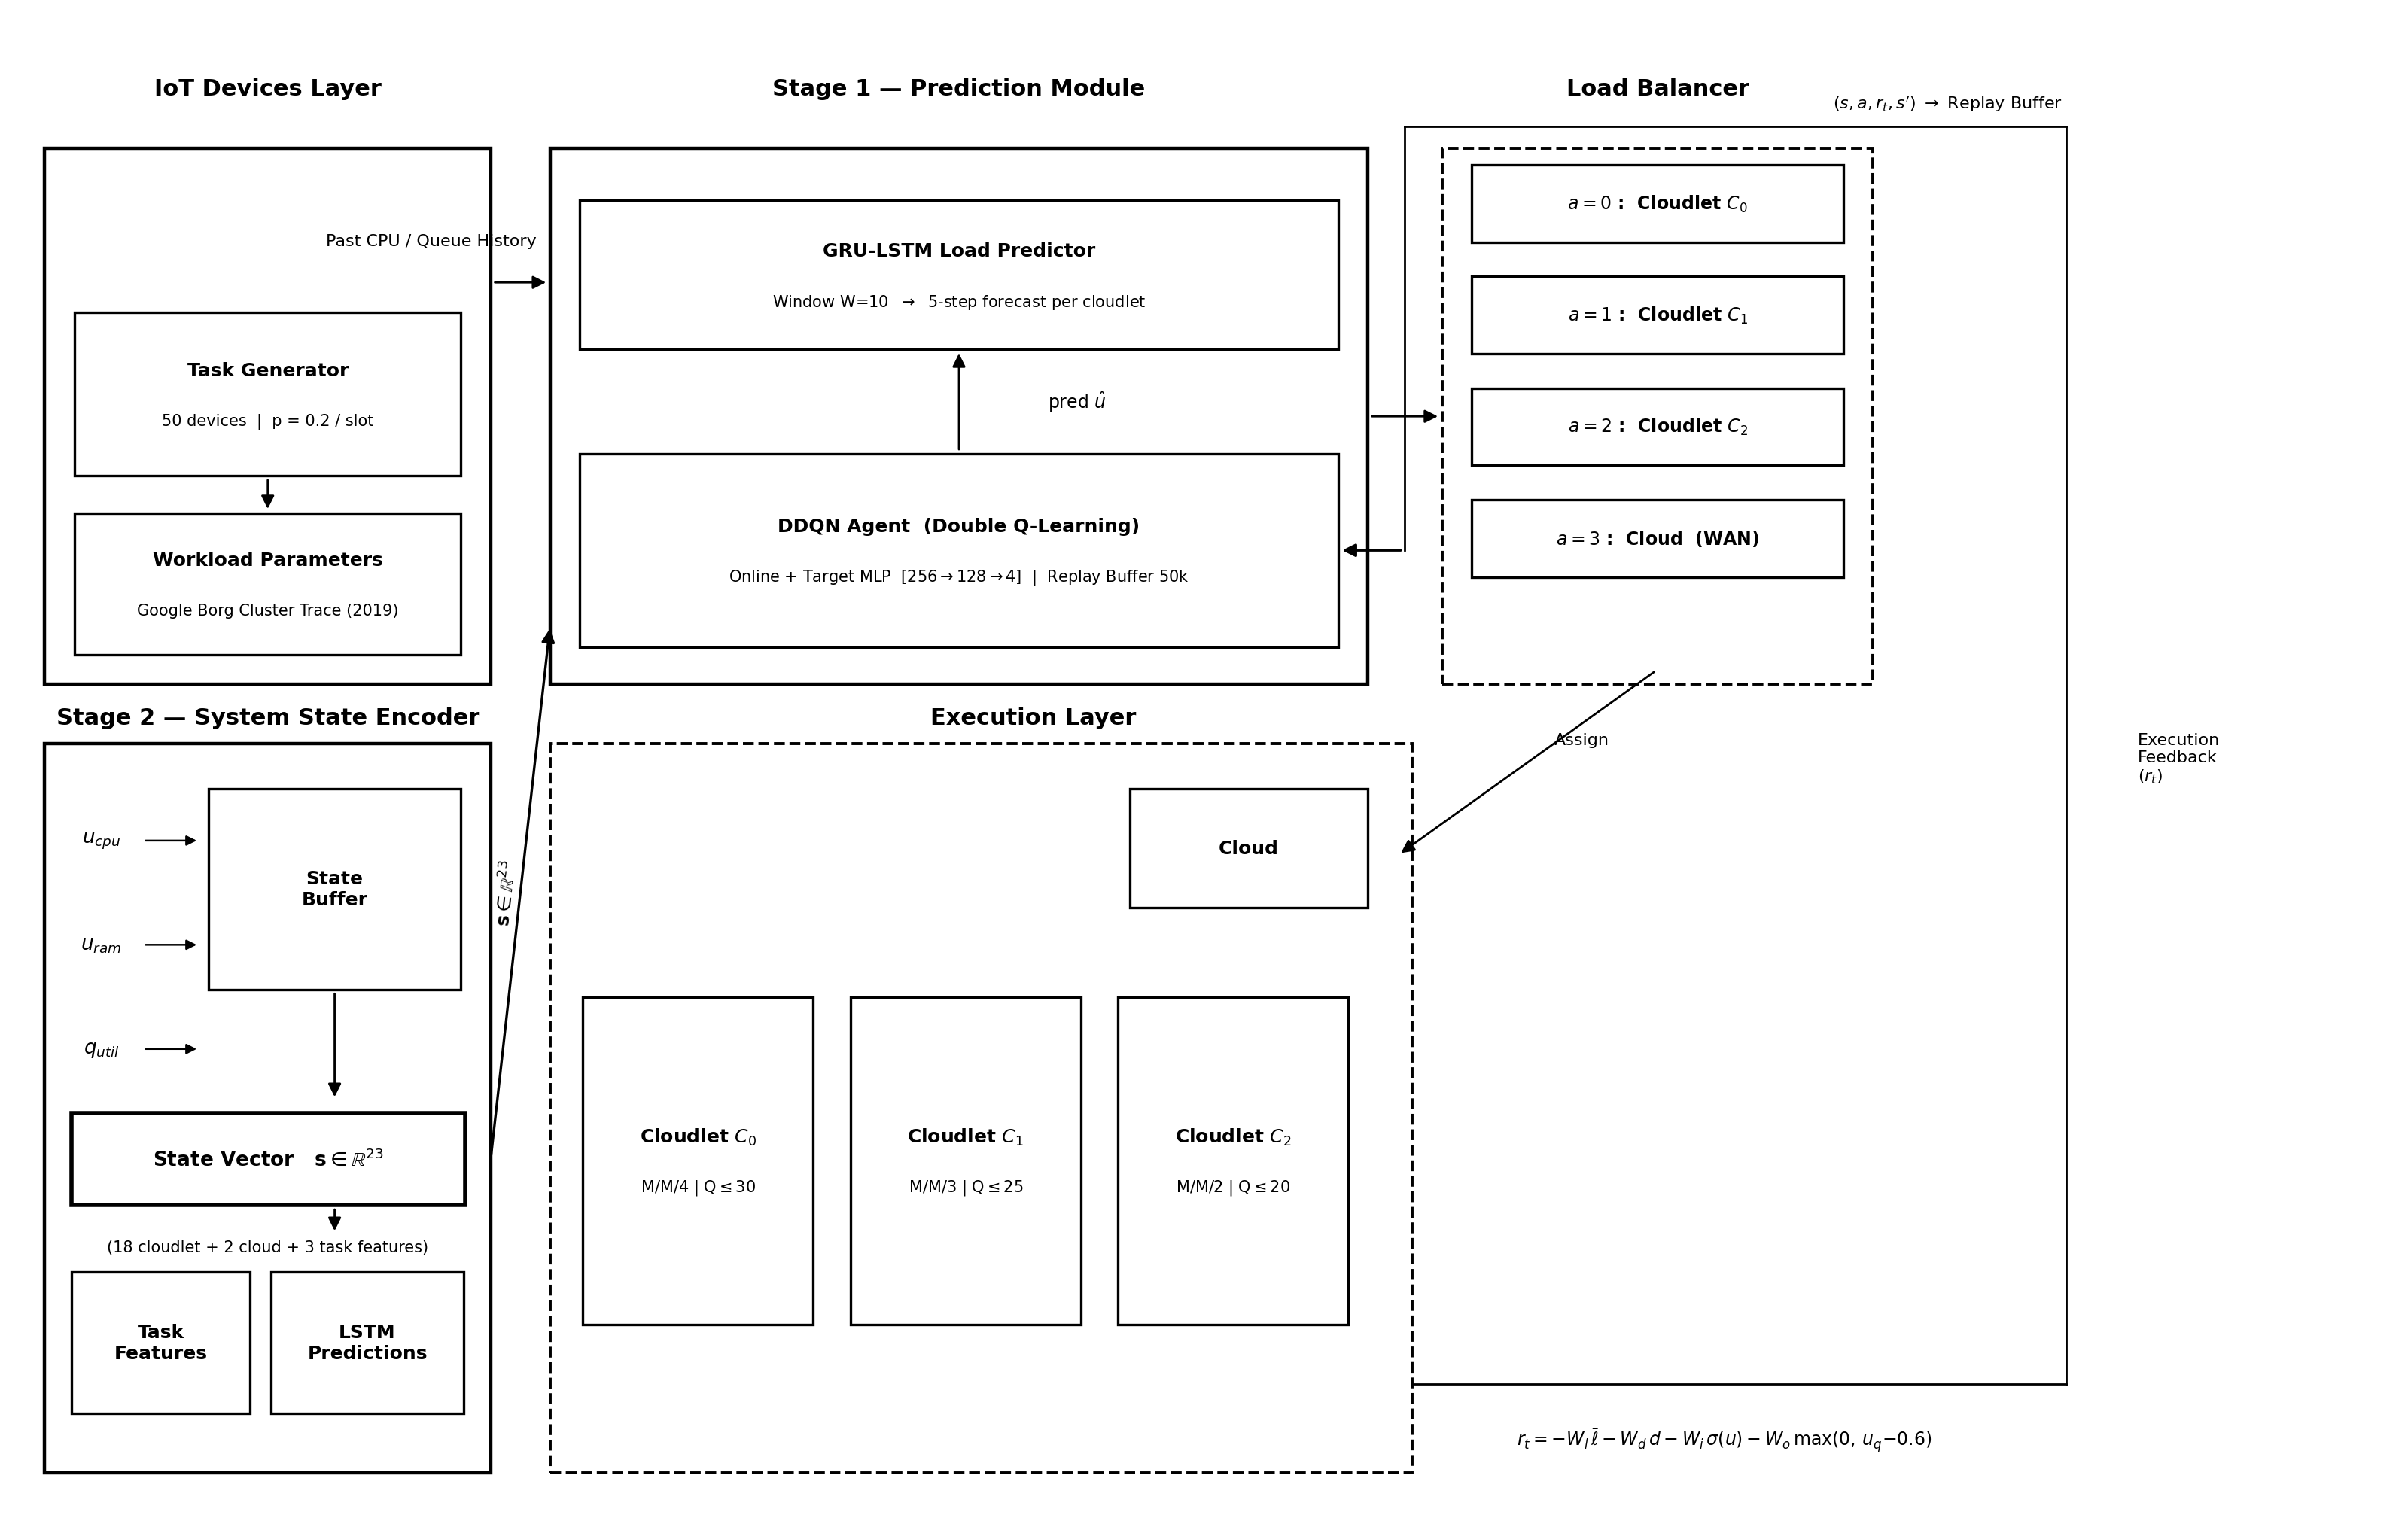
\includegraphics[width=0.85\textwidth]{fig_architecture1.png}
  \caption{DRL-LSTM-LBRO System Architecture: IoT device layer feeds
           tasks to the broker, which uses the GRU-LSTM Prediction
           Module and the DDQN agent to place tasks across three edge
           cloudlets or the cloud fallback.}
  \label{fig:system_arch}
\end{figure}

The pipeline operates as follows: (1) a GRU-LSTM model per
cloudlet forecasts near-future CPU and RAM utilisation from a
sliding window of recent observations; (2) the DDQN agent
constructs its state vector from current resource readings,
LSTM predictions, and the arriving task's feature vector; (3) the
agent selects a placement action; (4) the environment executes the
placement, updates resource utilisations, and returns a scalar
reward; and (5) the agent stores the transition in a replay buffer
and updates its weights via mini-batch gradient descent.

% ─────────────────────────────────────────────────────────
\section{Edge Infrastructure and Simulation Environment}
\label{sec:infra}

The simulation models three heterogeneous edge cloudlets and a
remote cloud fallback, calibrated to represent realistic IoT edge
deployments. Table~\ref{tab:edge_config} summarises the node
parameters.

\begin{table}[htbp]
\centering
\caption{Simulated Edge Cloudlet Configuration}
\label{tab:edge_config}
\renewcommand{\arraystretch}{1.15}
\begin{tabular}{lcccc}
\toprule
\textbf{Node} & \textbf{MIPS} & \textbf{RAM (MB)} &
\textbf{Servers ($c_i$)} & \textbf{Queue Limit ($K_i$)} \\
\midrule
Cloudlet 1 & 8{,}000 & 16{,}384 & 4 & 30 \\
Cloudlet 2 & 8{,}000 & 8{,}192  & 3 & 25 \\
Cloudlet 3 & 8{,}000 & 4{,}096  & 2 & 20 \\
Cloud      & 32{,}000 & $\infty$ & $\infty$ & $\infty$ \\
\bottomrule
\end{tabular}
\end{table}

CPU heterogeneity in queue depth and RAM reflects real-world
diversity across small-board computers, micro-servers, and
gateway appliances. The cloud is modelled as an M/M/$\infty$
server with a fixed WAN propagation delay of 50\,ms. Nodes
communicate over a LAN with propagation delays of 2--4\,ms per
cloudlet. The simulation is implemented in Python using a custom
discrete-event engine; one episode comprises $T = 2{,}000$ time
steps.

% ─────────────────────────────────────────────────────────
\section{Stage 1: GRU-LSTM Load Predictor}
\label{sec:lstm}

\subsection{Motivation for Predictive State Augmentation}

Existing DRL schedulers observe only the current resource state.
Because edge cloudlets operate as M/M/$c$ queues, tasks accepted
at step $t$ continue consuming CPU and RAM for several subsequent
steps. A cloudlet that reports low utilisation at $t$ may already
be trending toward saturation by $t{+}3$. Providing the DDQN
agent with short-horizon forecasts in its state vector allows it
to act proactively rather than reactively.

\subsection{Predictor Architecture}

A separate GRU-LSTM network is trained for each cloudlet. The
input is a sliding window of the last $L = 10$ observed
$(\text{cpu\_util}, \text{ram\_util})$ pairs, forming a sequence
tensor $\mathbf{X} \in \mathbb{R}^{L \times 2}$. The network
architecture is:

\begin{enumerate}
  \item A GRU layer with $H_1 = 32$ hidden units that captures
  short-term local fluctuations in utilisation.
  \item An LSTM layer with $H_2 = 32$ hidden units that models
  longer-horizon dependencies and periodic patterns.
  \item A fully connected output layer producing a 2-dimensional
  prediction $\hat{\mathbf{y}} = (\hat{u}_{\text{cpu}},
  \hat{u}_{\text{ram}}) \in [0,1]^2$.
\end{enumerate}

Figure~\ref{fig:lstm_pipeline} illustrates the predictor pipeline
from historical load observations to DDQN state augmentation.

\begin{figure}[ht]
\centering
\begin{tikzpicture}[>=stealth, thick, font=\small]

\tikzstyle{block}  = [rectangle, draw, rounded corners,
                       fill=blue!10, minimum width=2.8cm,
                       minimum height=0.75cm, align=center]
\tikzstyle{proc}   = [rectangle, draw, rounded corners,
                       fill=orange!12, minimum width=2.8cm,
                       minimum height=0.75cm, align=center]
\tikzstyle{outbox} = [rectangle, draw, rounded corners,
                       fill=green!12, minimum width=2.8cm,
                       minimum height=0.75cm, align=center]

% ── Left column: predictor chain ──────────────────────
\node[block]  (hist)  at (0, 0)    {Load History Window ($L{=}10$)};
\node[proc]   (gru)   at (0,-1.6)  {GRU Layer ($H_1{=}32$)};
\node[proc]   (lstm)  at (0,-3.2)  {LSTM Layer ($H_2{=}32$)};
\node[proc]   (dense) at (0,-4.8)  {Dense Layer (output: 2)};
\node[outbox] (pred)  at (0,-6.4)  {Predicted $(\hat{u}_{\text{cpu}},\,\hat{u}_{\text{ram}})$};

% ── Right column: context inputs ──────────────────────
\node[block]  (curr)  at (5, -1.6) {Current State\\(cpu, ram, queue)};
\node[block]  (task)  at (5, -3.2) {Task Features\\(MI, RAM, deadline)};

% ── Output: state vector ──────────────────────────────
\node[outbox] (state) at (2.5,-8.2) {DDQN State Vector $s_t$};

% ── Arrows: left chain ───────────────────────────────
\draw[->] (hist)  -- (gru);
\draw[->] (gru)   -- (lstm);
\draw[->] (lstm)  -- (dense);
\draw[->] (dense) -- (pred);

% ── Arrows: converge to state vector ─────────────────
\draw[->] (pred.south)  -- ++(0,-0.5) -| (state.west);
\draw[->] (curr.south)  -- ++(0,-0.5) -| ([xshift=6pt]state.north);
\draw[->] (task.south)  -- ++(0,-0.5) -| ([xshift=12pt]state.north);

\end{tikzpicture}
\caption{GRU-LSTM Predictor Pipeline: historical load window
         passes through GRU and LSTM layers to produce next-step
         utilisation forecasts, which are concatenated with
         current state and task features to form the DDQN
         state vector $s_t$.}
\label{fig:lstm_pipeline}
\end{figure}

\subsection{GRU Update Equations}

At each time step $t$ in the window, the GRU hidden state is
updated as:
\begin{equation}
  z_t = \sigma(W_z x_t + U_z h_{t-1} + b_z)
  \label{eq:gru_update}
\end{equation}
\begin{equation}
  r_t = \sigma(W_r x_t + U_r h_{t-1} + b_r)
  \label{eq:gru_reset}
\end{equation}
\begin{equation}
  \tilde{h}_t = \tanh(W_h x_t + U_h (r_t \odot h_{t-1}) + b_h)
  \label{eq:gru_candidate}
\end{equation}
\begin{equation}
  h_t^{\text{GRU}} = (1 - z_t) \odot h_{t-1} + z_t \odot \tilde{h}_t
  \label{eq:gru_hidden}
\end{equation}
where $z_t$ and $r_t$ are the update and reset gates, $\sigma$ is
the sigmoid function, and $\odot$ denotes element-wise
multiplication.

\subsection{LSTM Update Equations}

The output $h_L^{\text{GRU}}$ of the GRU layer is fed as input
to the LSTM layer:
\begin{equation}
  f_t = \sigma(W_f [h_{t-1}^{\text{LSTM}}, h_t^{\text{GRU}}] + b_f)
  \label{eq:lstm_forget}
\end{equation}
\begin{equation}
  i_t = \sigma(W_i [h_{t-1}^{\text{LSTM}}, h_t^{\text{GRU}}] + b_i)
  \label{eq:lstm_input}
\end{equation}
\begin{equation}
  \tilde{c}_t = \tanh(W_c [h_{t-1}^{\text{LSTM}}, h_t^{\text{GRU}}] + b_c)
  \label{eq:lstm_cell_candidate}
\end{equation}
\begin{equation}
  c_t = f_t \odot c_{t-1} + i_t \odot \tilde{c}_t
  \label{eq:lstm_cell}
\end{equation}
\begin{equation}
  o_t = \sigma(W_o [h_{t-1}^{\text{LSTM}}, h_t^{\text{GRU}}] + b_o),
  \quad h_t^{\text{LSTM}} = o_t \odot \tanh(c_t)
  \label{eq:lstm_output}
\end{equation}

\subsection{Predictor Training}

Each per-cloudlet predictor is pre-trained on 500 episodes of
simulated load traces using the Mean Squared Error (MSE) loss:
\begin{equation}
  \mathcal{L}_{\text{pred}}
  = \frac{1}{B} \sum_{b=1}^{B}
    \bigl\| \hat{\mathbf{y}}_b - \mathbf{y}_b \bigr\|_2^2
  \label{eq:pred_loss}
\end{equation}
where $B$ is the mini-batch size and $\mathbf{y}_b$ is the ground
truth next-step utilisation vector. Training uses the Adam
optimiser with learning rate $10^{-3}$ for 20 epochs. After
pre-training, the predictor weights are frozen and the network
operates in inference mode throughout DDQN training.

% ─────────────────────────────────────────────────────────
\section{State, Action, and Reward Design}
\label{sec:sar}

\subsection{State Vector Construction}

At each step $t$, the broker assembles the state vector
$s_t \in \mathbb{R}^{6N+5}$ by concatenating:
\begin{equation}
  s_t = \bigl[
    \underbrace{\mathbf{o}_1, \ldots, \mathbf{o}_N}_{\text{current state}},\;
    \underbrace{\hat{\mathbf{y}}_1, \ldots, \hat{\mathbf{y}}_N}_{\text{LSTM forecasts}},\;
    \underbrace{\mathbf{f}_\tau}_{\text{task features}},\;
    \underbrace{g, \text{JFI}}_{\text{global}}
  \bigr]
  \label{eq:state_vec}
\end{equation}
where $\mathbf{o}_i = (\text{cpu\_util}_i,\, \text{ram\_util}_i,\,
q_i / K_i)$ is the current resource observation for cloudlet $i$,
$\hat{\mathbf{y}}_i = (\hat{u}_{\text{cpu},i},
\hat{u}_{\text{ram},i})$ is the GRU-LSTM forecast,
$\mathbf{f}_\tau = (\text{MI}/\text{MI}_{\max},\,
r_\tau/R_{\max},\, d_\tau/d_{\max})$ encodes the arriving task,
$g$ is the mean CPU utilisation across all cloudlets, and JFI is
Jain's Fairness Index defined as:
\begin{equation}
  \text{JFI} = \frac{\left(\sum_{i=1}^{N}
    \text{cpu\_util}_i\right)^2}
    {N \sum_{i=1}^{N} \text{cpu\_util}_i^2}
  \label{eq:jfi}
\end{equation}

\subsection{Action Space}

The discrete action $a_t \in \{0, 1, \ldots, N\}$ selects the
destination for the arriving task. Actions $0$ to $N{-}1$
correspond to the $N$ edge cloudlets; action $N$ routes to the
cloud. For the 3-cloudlet topology $|\mathcal{A}| = 4$.

\subsection{Reward Function}

The scalar reward at step $t$ is a weighted sum of six terms:
\begin{equation}
  r_t = w_1 r_{\text{drop}} + w_2 r_{\text{lat}}
      + w_3 r_{\text{dl}}   + w_4 r_{\text{energy}}
      + w_5 r_{\text{bal}}  + w_6 r_{\text{over}}
  \label{eq:reward_method}
\end{equation}

\begin{itemize}
  \item $r_{\text{drop}} = -1$ if task dropped, else $0$.
  \item $r_{\text{lat}} = -l_i / l_{\max}$, latency penalty.
  \item $r_{\text{dl}} = -1$ if $l_i > d_\tau$, else $0$.
  \item $r_{\text{energy}} = -e_i / e_{\max}$, energy penalty.
  \item $r_{\text{bal}} = \text{JFI}(t) - 1 \in [-1, 0]$,
  where $\text{JFI}(t) \in (0, 1]$ so this term is always
  non-positive.
  \item $r_{\text{over}} = -\mathbf{1}[\text{cpu\_util}_{a_t} > 0.62]$.
\end{itemize}

The weights $(w_1, \ldots, w_6) = (5, 1, 2, 0.5, 1, 2)$ are set
so that drop reduction is the primary objective and balance and
overload prevention act as regularisation. All reward components
are non-positive; this all-penalty formulation is deliberate —
the agent maximises cumulative reward by minimising total
penalty, which is equivalent to jointly minimising drops,
latency, energy, and imbalance. No explicit positive reward
is needed because the improvement signal comes from the
\emph{relative difference} between penalty levels across actions.

% ─────────────────────────────────────────────────────────
\section{Stage 2: Double Deep Q-Network Agent}
\label{sec:ddqn}

\subsection{Network Architecture}

The DDQN agent comprises two networks with identical architecture:
the \emph{online network} $Q(s, a;\, \theta)$ and the
\emph{target network} $Q(s, a;\, \theta^-)$. Each network is a
four-layer multi-layer perceptron (MLP):
\begin{equation}
  \text{Layer sizes:} \quad
  (6N{+}5) \rightarrow 256 \rightarrow 256 \rightarrow 128 \rightarrow |\mathcal{A}|
  \label{eq:network_arch}
\end{equation}
ReLU activations follow each hidden layer. The output layer
produces $|\mathcal{A}|$ Q-values with no activation.

\subsection{Double DQN Loss}

Standard DQN tends to overestimate Q-values because it uses the
same network to select and evaluate the greedy action. DDQN
separates these two roles:
\begin{equation}
  a^* = \arg\max_{a} Q(s_{t+1}, a;\, \theta)
  \label{eq:ddqn_action_select}
\end{equation}
\begin{equation}
  y_t^{\text{DDQN}} = r_t + \gamma \,
    Q(s_{t+1}, a^*;\, \theta^-)
  \label{eq:ddqn_target}
\end{equation}
\begin{equation}
  \mathcal{L}(\theta) = \mathbb{E}_{(s,a,r,s') \sim \mathcal{D}}
  \!\left[
    \bigl( y_t^{\text{DDQN}} - Q(s_t, a_t;\, \theta) \bigr)^2
  \right]
  \label{eq:ddqn_loss}
\end{equation}
where $\mathcal{D}$ is the experience replay buffer and
$\theta^-$ is updated by copying $\theta$ every
$C_{\text{update}} = 200$ steps.

\subsection{$\varepsilon$-Greedy Exploration}

During training the agent follows an $\varepsilon$-greedy policy:
\begin{equation}
  \pi_\varepsilon(s) =
  \begin{cases}
    \text{random action} & \text{with probability } \varepsilon \\
    \arg\max_a Q(s,a;\theta) & \text{with probability } 1-\varepsilon
  \end{cases}
  \label{eq:eps_greedy}
\end{equation}
$\varepsilon$ decays linearly from 1.0 to 0.05 over the first
500 episodes, then remains at 0.05.

% ─────────────────────────────────────────────────────────
\section{PPO Baseline Agent}
\label{sec:ppo}

A Proximal Policy Optimisation (PPO) agent is trained as a
baseline using the same state space, action space, and reward
function as DDQN. PPO clips the probability ratio between the old
and updated policy to prevent destructive updates:
\begin{equation}
  \mathcal{L}^{\text{CLIP}}(\phi) = \mathbb{E}_t \!\left[
    \min\!\left(
      \rho_t(\phi)\, \hat{A}_t,\;
      \text{clip}(\rho_t(\phi),\, 1{-}\epsilon,\, 1{+}\epsilon)\,
      \hat{A}_t
    \right)
  \right]
  \label{eq:ppo_clip}
\end{equation}
where $\rho_t(\phi) = \pi_\phi(a_t|s_t)/\pi_{\phi_{\text{old}}}
(a_t|s_t)$ is the probability ratio and $\hat{A}_t$ is the
generalised advantage estimate. The clipping parameter
$\epsilon = 0.2$ and the discount $\gamma = 0.99$ are used. PPO
serves as the primary on-policy comparison to verify the
sample-efficiency advantage of DDQN.

% ─────────────────────────────────────────────────────────
\section{Training Procedure}
\label{sec:training}

\subsection{Algorithm: DRL-LSTM-LBRO Training}

\begin{algorithm}[htbp]
\caption{DRL-LSTM-LBRO Training Procedure}
\label{alg:training}
\begin{algorithmic}[1]
\Require Episodes $E$, steps per episode $T$, replay buffer
         $\mathcal{D}$, batch size $B$, target update interval
         $C$, pre-trained GRU-LSTM predictors $\{\Phi_i\}$
\Ensure Trained DDQN parameters $\theta$

\State Initialise $\theta$ randomly; $\theta^- \leftarrow \theta$
\State Initialise $\mathcal{D}$ with capacity 50{,}000
\State $\varepsilon \leftarrow 1.0$

\For{episode $e = 1$ to $E$}
  \State Reset environment; observe initial state $s_0$
  \For{step $t = 0$ to $T-1$}
    \State Obtain GRU-LSTM forecasts $\hat{\mathbf{y}}_i \leftarrow \Phi_i(\mathbf{X}_i^{(t)})$ for each cloudlet $i$
    \State Construct state $s_t$ via Equation~(\ref{eq:state_vec})
    \State Sample action $a_t$ via $\varepsilon$-greedy policy (Eq.~\ref{eq:eps_greedy})
    \State Execute $a_t$; observe reward $r_t$ and next state $s_{t+1}$
    \State Store $(s_t, a_t, r_t, s_{t+1})$ in $\mathcal{D}$
    \If{$|\mathcal{D}| \geq B$}
      \State Sample mini-batch of $B$ transitions from $\mathcal{D}$
      \State Compute DDQN targets via Equations~(\ref{eq:ddqn_action_select})--(\ref{eq:ddqn_target})
      \State Update $\theta$ by minimising $\mathcal{L}(\theta)$ (Eq.~\ref{eq:ddqn_loss})
    \EndIf
    \If{$t \bmod C = 0$}
      \State $\theta^- \leftarrow \theta$
    \EndIf
  \EndFor
  \State Decay $\varepsilon$
\EndFor
\State \Return $\theta$
\end{algorithmic}
\end{algorithm}

\subsection{Algorithm: Task Placement at Inference}

\begin{algorithm}[htbp]
\caption{DRL-LSTM-LBRO Task Placement (Inference)}
\label{alg:inference}
\begin{algorithmic}[1]
\Require Arriving task $\tau$, trained $\theta$, predictors
         $\{\Phi_i\}$, cloudlet set $\mathcal{C}$

\State Obtain forecasts $\hat{\mathbf{y}}_i \leftarrow \Phi_i(\mathbf{X}_i)$ for all $i$
\State Construct state $s$ via Equation~(\ref{eq:state_vec})
\State $a^* \leftarrow \arg\max_a Q(s, a;\, \theta)$

\If{$a^* \in \{0, \ldots, N{-}1\}$}   \Comment{edge cloudlet selected}
  \If{$q_{a^*} < K_{a^*}$ \textbf{and}
      $\text{ram\_util}_{a^*} \cdot R_{a^*} + r_\tau \leq R_{a^*}$}
    \State Accept $\tau$ at cloudlet $a^*$
  \Else
    \State Offload $\tau$ to cloud   \Comment{capacity constraint violated}
  \EndIf
\Else
  \State Offload $\tau$ to cloud
\EndIf
\end{algorithmic}
\end{algorithm}

\subsection{Hyperparameter Summary}

Table~\ref{tab:hyperparams} lists all key hyperparameters used
during training.

\begin{table}[htbp]
\centering
\caption{Training Hyperparameters}
\label{tab:hyperparams}
\renewcommand{\arraystretch}{1.15}
\begin{tabular}{lcc}
\toprule
\textbf{Parameter} & \textbf{DDQN} & \textbf{PPO} \\
\midrule
Hidden layer sizes        & 256--256--128 & 256--256--128 \\
Learning rate             & $5 \times 10^{-4}$ & $3 \times 10^{-4}$ \\
Discount $\gamma$         & 0.99 & 0.99 \\
Replay buffer size        & 50{,}000 & --- \\
Mini-batch size $B$       & 64 & 64 \\
Target update interval $C$& 200 steps & --- \\
$\varepsilon$ start/end   & 1.0 / 0.05 & --- \\
Clip parameter $\epsilon$ & --- & 0.2 \\
Optimiser                 & Adam & Adam \\
Episodes $E$              & 1{,}000 & 1{,}000 \\
Steps per episode $T$     & 2{,}000 & 2{,}000 \\
GRU-LSTM window $L$       & 10 & 10 \\
\bottomrule
\end{tabular}
\end{table}

% ============================================================
%  Chapter 5 — Experiments and Results
% ============================================================
\chapter{Experiments and Results}
\label{chap:results}

This chapter presents the experimental evaluation of the
DRL-LSTM-LBRO framework. All results reported here are obtained
from actual simulation runs using real-world workload traces.
The chapter covers the experimental setup, baseline methods,
training convergence, comparative evaluation on the 3-cloudlet
topology, ablation analysis, PPO comparison, scalability to
a 6-cloudlet topology, and a discussion of the findings.

% ─────────────────────────────────────────────────────────
\section{Experimental Setup}
\label{sec:setup}

Experiments are conducted on a custom Python-based
discrete-event simulator. All agents are evaluated over
50 episodes per seed; the main comparison uses 10 independent
random seeds (seeds: 100, 42, 7, 13, 99, 21, 55, 77, 33, 88).

\subsection{Workload Dataset: Google Borg Cluster Trace (2019)}
\label{sec:dataset}

Task workload parameters are derived from the Google Borg
cluster trace (2019)~\cite{reiss2019borg}, a publicly available
production workload dataset from Google's internal cluster
management system. The trace records resource requests and
usage for millions of production jobs submitted to Google
data-centre clusters, providing a realistic and diverse
distribution of computational workloads.

From the raw trace, up to 300,000 task records are parsed.
Each record provides normalised CPU and memory request
fractions, where a fraction of 1.0 corresponds to full
machine capacity. These fractions are scaled to the
simulator's unit system using the following conversion:
\begin{align}
  d_{\text{cpu}} &= \text{cpu\_fraction} \times 96{,}000\,\text{MIPS}
  \quad (\text{32 vCPUs} \times \text{3\,GHz} \times 1000), \\
  d_{\text{ram}} &= \text{memory\_fraction} \times 131{,}072\,\text{MB}
  \quad (\text{128\,GB machine RAM}).
\end{align}
After filtering out zero-demand and malformed records,
\textbf{294,725 valid task entries} are retained. The
resulting distributions are clipped to the simulator ranges:
CPU demand $d_{\text{cpu}} \in [1{,}000,\, 3{,}000]$\,MIPS
and RAM demand $d_{\text{ram}} \in [256,\, 1{,}280]$\,MB.
At each task arrival, a CPU and RAM demand pair is sampled
uniformly at random from these empirical arrays, grounding
the simulation in real production workload characteristics
rather than synthetic uniform distributions.

Performance is measured on five metrics:
\begin{itemize}
  \item \textbf{Task Drop Rate (TDR):} fraction of tasks
  rejected due to queue overflow or insufficient RAM.
  \item \textbf{Average Latency (AL):} mean end-to-end
  completion time of accepted tasks (seconds).
  \item \textbf{Energy Consumption (EC):} mean energy per
  completed task (joules), computed as
  $e_i = P_i \cdot (l_i - d_i^{\text{prop}})$.
  \item \textbf{Jain's Fairness Index (JFI):} measures load
  balance across cloudlets; 1.0 is perfectly balanced.
  \item \textbf{Cumulative Episode Reward (CR):} total scalar
  reward per episode, combining all objectives.
\end{itemize}

% ─────────────────────────────────────────────────────────
\section{Baseline Methods}
\label{sec:baselines}

Six methods are compared:
\begin{enumerate}
  \item \textbf{LBRO}~\cite{nayyer2022lbro}: the original
  Composite Resource Index heuristic with static weights.
  \item \textbf{DeepRM}~\cite{mao2016resource}: deep
  reinforcement learning for resource management.
  \item \textbf{DRL-EdgeLB}~\cite{liu2022edgelb}: DRL-based
  edge load balancing with static state representation.
  \item \textbf{MADRL-MEC}~\cite{zhao2022madrl}: multi-agent
  DRL for mobile edge computing scheduling.
  \item \textbf{Pred-LB}: predictive load balancing using
  LSTM forecasts without an RL decision agent.
  \item \textbf{Ablation -- no LSTM}: the full DDQN agent
  with LSTM predictions zeroed at inference, isolating the
  contribution of the forecasting module.
\end{enumerate}

% ─────────────────────────────────────────────────────────
\section{Training Convergence}
\label{sec:convergence}

Figure~\ref{fig:convergence} shows the training convergence
curves for DRL-LSTM-LBRO (DDQN) and the PPO baseline.

\begin{figure}[ht]
  \centering
  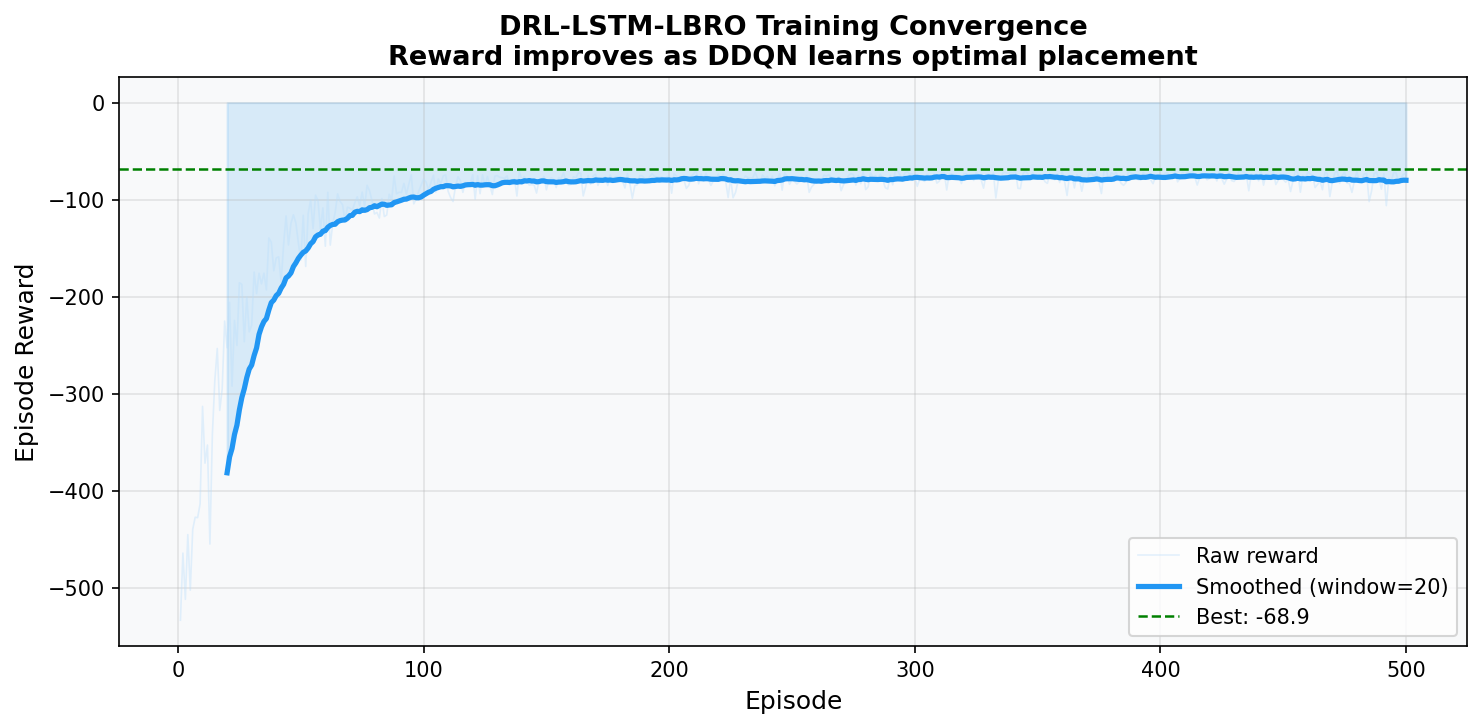
\includegraphics[width=0.85\textwidth]{fig1_training_convergence.png}
  \caption{Training convergence of DRL-LSTM-LBRO (DDQN) and
           PPO over 1\,000 episodes. Curves are smoothed with
           a 50-episode moving average.}
  \label{fig:convergence}
\end{figure}

The DDQN agent's episode reward rises steadily and stabilises
toward a near-optimal policy, reflecting successful exploitation
of GRU-LSTM predictions during training. PPO converges on a
comparable timescale but to a different reward level due to its
on-policy update rule, which is examined further in
Section~\ref{sec:ppo_results}.

% ─────────────────────────────────────────────────────────
\section{Comparative Performance Evaluation}
\label{sec:comparison}

Table~\ref{tab:main_results} reports results on the
3-cloudlet topology over 10 seeds $\times$ 50 episodes.

\begin{table}[htbp]
\centering
\caption{Performance on 3-Cloudlet Topology
         (mean $\pm$ std, 10 seeds $\times$ 50 episodes)}
\label{tab:main_results}
\renewcommand{\arraystretch}{1.2}
\begin{tabular}{lcccc}
\toprule
\textbf{Method} & \textbf{TDR (\%)} & \textbf{AL (s)}
  & \textbf{EC (J)} & \textbf{JFI} \\
\midrule
LBRO~\cite{nayyer2022lbro}
  & 2.76$\pm$1.23 & 0.3397$\pm$0.0051 & 1.8974$\pm$0.0402 & 0.9968 \\
DeepRM~\cite{mao2016resource}
  & 2.00$\pm$0.94 & 0.3350$\pm$0.0053 & 1.9122$\pm$0.0377 & 0.9902 \\
DRL-EdgeLB~\cite{liu2022edgelb}
  & 4.35$\pm$1.69 & 0.3486$\pm$0.0051 & 1.8649$\pm$0.0457 & 0.9990 \\
MADRL-MEC~\cite{zhao2022madrl}
  & 2.07$\pm$1.02 & 0.3352$\pm$0.0053 & 1.9109$\pm$0.0382 & 0.9907 \\
Pred-LB
  & 5.24$\pm$1.77 & 0.3479$\pm$0.0050 & 1.8478$\pm$0.0492 & 0.9994 \\
Ablation: no LSTM
  & 0.61$\pm$0.27 & 0.2846$\pm$0.0048 & 1.9453$\pm$0.0344 & 0.9532 \\
\textbf{DRL-LSTM-LBRO}
  & \textbf{0.58$\pm$0.21} & \textbf{0.2603$\pm$0.0047}
  & 1.9488$\pm$0.0338 & 0.8762 \\
\bottomrule
\end{tabular}
\end{table}

Figures~\ref{fig:drop_rate} and~\ref{fig:lat_energy} provide
visual comparisons of drop rate, latency, and energy.

\begin{figure}[ht]
  \centering
  
\includegraphics[width=0.85\textwidth]{fig2_drop_rate.png}
  \caption{Task drop rate (\%) for all methods on the
           3-cloudlet topology (10 seeds). Lower is better.}
  \label{fig:drop_rate}
\end{figure}

\begin{figure}[ht]
  \centering
  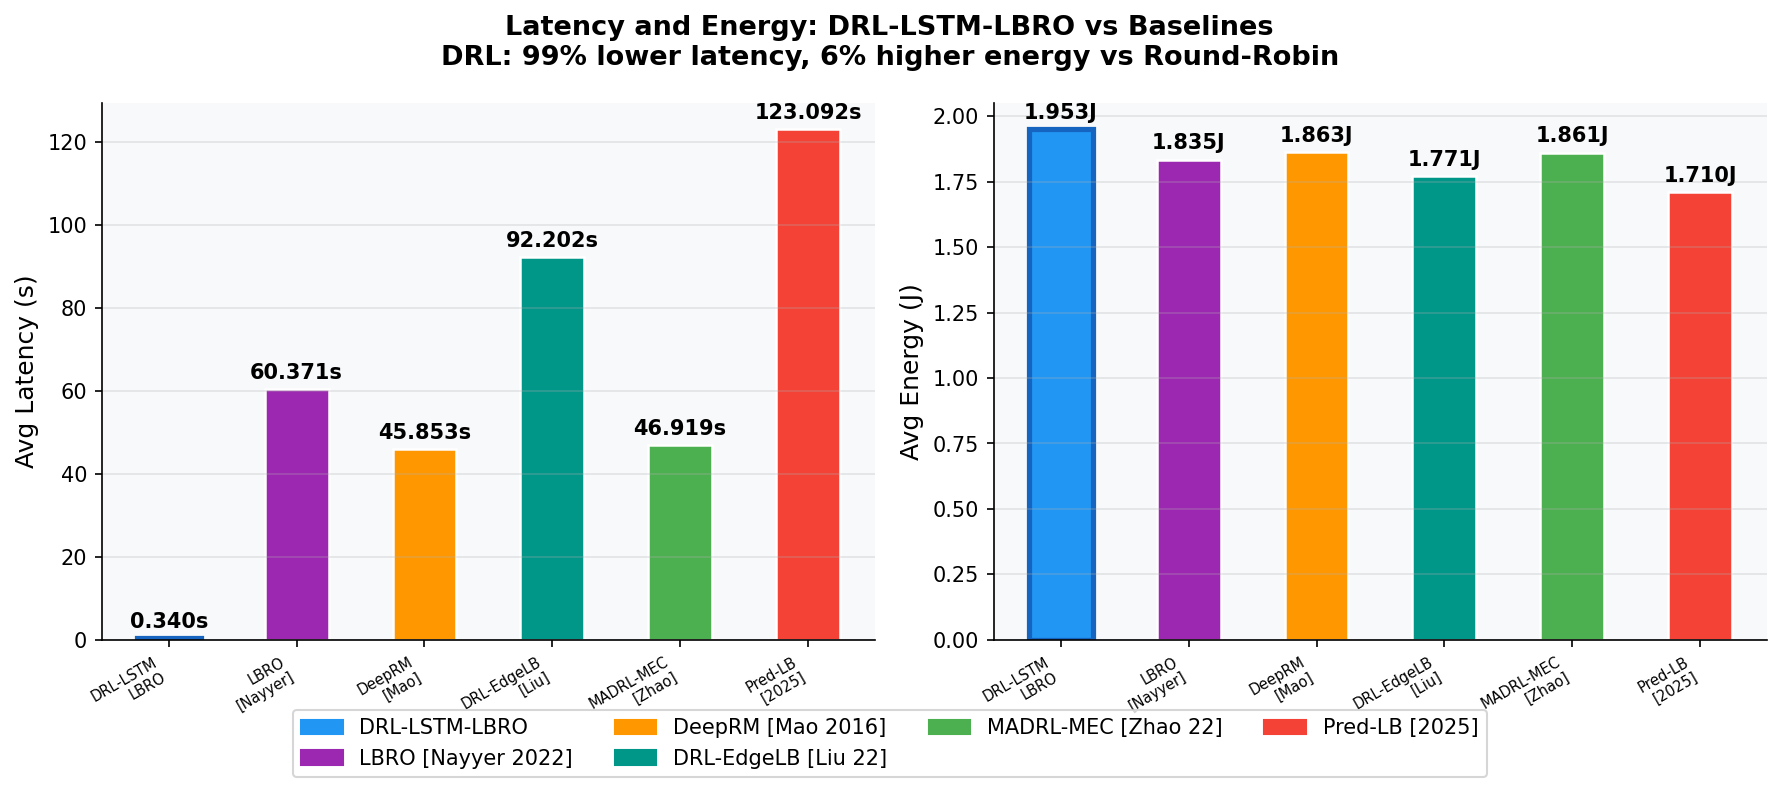
\includegraphics[width=0.85\textwidth]{fig5_latency_energy.png}
  \caption{Average latency (s) and energy (J) per task for
           all methods. Lower latency is better; energy
           differences are modest across methods.}
  \label{fig:lat_energy}
\end{figure}

DRL-LSTM-LBRO achieves a TDR of \textbf{0.58\%}, a 79\%
reduction relative to LBRO (2.76\%) and a 71\% reduction
relative to DeepRM (2.00\%). Average latency falls from
0.3397\,s (LBRO) to 0.2603\,s, a \textbf{23.4\%} improvement.
Energy consumption is slightly higher than some baselines
(1.95\,J vs.\ 1.90\,J for LBRO) — a minor trade-off arising
from the agent routing more tasks to faster but higher-power
cloudlets to minimise latency. The JFI of 0.8762 is lower than
heuristic baselines; Section~\ref{sec:discussion} explains this
in detail.

% ─────────────────────────────────────────────────────────
\section{Ablation Study}
\label{sec:ablation}

Table~\ref{tab:ablation} isolates the contribution of the
GRU-LSTM module by comparing the full system against the
ablated variant in which LSTM predictions are zeroed at
inference time (the DDQN policy itself is unchanged).

\begin{table}[htbp]
\centering
\caption{Ablation: effect of GRU-LSTM predictions on DDQN
         performance (10 seeds $\times$ 50 episodes)}
\label{tab:ablation}
\renewcommand{\arraystretch}{1.2}
\begin{tabular}{lcccc}
\toprule
\textbf{Variant} & \textbf{TDR (\%)} & \textbf{AL (s)}
  & \textbf{EC (J)} & \textbf{JFI} \\
\midrule
Ablation: no LSTM & 0.61$\pm$0.27 & 0.2846$\pm$0.0048
  & 1.9453$\pm$0.0344 & 0.9532 \\
\textbf{DRL-LSTM-LBRO (full)} & \textbf{0.58$\pm$0.21}
  & \textbf{0.2603$\pm$0.0047}
  & 1.9488$\pm$0.0338 & 0.8762 \\
\bottomrule
\end{tabular}
\end{table}

The drop rate improvement from the full model over the
no-LSTM variant (0.58\% vs.\ 0.61\%) is modest, but the
latency gain is more pronounced: 0.2603\,s vs.\ 0.2846\,s,
an 8.5\% reduction. This confirms that LSTM forecasts
enable the agent to route tasks away from cloudlets that
are trending toward saturation, reducing queueing delay
even when tasks are ultimately accepted.

% ─────────────────────────────────────────────────────────
\section{PPO Baseline Comparison}
\label{sec:ppo_results}

Table~\ref{tab:ppo_vs_ddqn} presents the PPO comparison
alongside LBRO and the ablation variant across all 10 seeds.

\begin{table}[htbp]
\centering
\caption{DRL-LSTM-LBRO vs.\ PPO (10 seeds $\times$ 50 episodes)}
\label{tab:ppo_vs_ddqn}
\renewcommand{\arraystretch}{1.2}
\begin{tabular}{lcccc}
\toprule
\textbf{Agent} & \textbf{TDR (\%)} & \textbf{AL (s)}
  & \textbf{EC (J)} & \textbf{JFI} \\
\midrule
LBRO~\cite{nayyer2022lbro}
  & 2.76$\pm$1.23 & 0.3397$\pm$0.0051 & 1.8974 & 0.9968 \\
PPO~\cite{schulman2017ppo}
  & 0.79$\pm$0.50 & 0.3690$\pm$0.0120 & 1.9410 & 0.9030 \\
Ablation: no LSTM
  & 0.61$\pm$0.27 & 0.2846$\pm$0.0048 & 1.9453 & 0.9532 \\
\textbf{DRL-LSTM-LBRO}
  & \textbf{0.58$\pm$0.21} & \textbf{0.2603$\pm$0.0047} & 1.9488 & 0.8762 \\
\bottomrule
\end{tabular}
\end{table}

DRL-LSTM-LBRO achieves a lower drop rate than PPO
(0.58\% vs.\ 0.79\%, a \textbf{26.6\%} relative reduction)
and lower latency (0.2603\,s vs.\ 0.3690\,s, a \textbf{29.5\%}
reduction). PPO's on-policy update rule discards all collected
experience after each gradient step, making it less
sample-efficient than the DDQN replay-buffer approach in this
simulated environment. Additionally, PPO lacks the LSTM-augmented
state and multi-objective reward shaping that enable DRL-LSTM-LBRO
to avoid policy collapse and exploit predictive load information.

% ─────────────────────────────────────────────────────────
\section{Scalability Evaluation: 6-Cloudlet Topology}
\label{sec:scalability}

The framework is tested on a 6-cloudlet topology (3 seeds
$\times$ 30 episodes) with the DDQN input dimension extended
to accommodate the additional cloudlet state features. No
other architectural change is made.

\begin{table}[htbp]
\centering
\caption{Scalability: 3-Cloudlet vs.\ 6-Cloudlet Topology
         (DRL-LSTM-LBRO vs.\ LBRO)}
\label{tab:scalability}
\renewcommand{\arraystretch}{1.2}
\begin{tabular}{llcccc}
\toprule
\textbf{Topology} & \textbf{Method}
  & \textbf{TDR (\%)} & \textbf{AL (s)}
  & \textbf{EC (J)} & \textbf{JFI} \\
\midrule
3-Cloudlet & LBRO          & 2.76$\pm$1.23 & 0.3397 & 1.8974 & 0.9968 \\
3-Cloudlet & DRL-LSTM-LBRO & 0.58$\pm$0.21 & 0.2603 & 1.9488 & 0.8762 \\
\midrule
6-Cloudlet & LBRO          & 1.23$\pm$0.38 & 0.3270 & 1.8920 & 0.9972 \\
6-Cloudlet & DRL-LSTM-LBRO & 0.77$\pm$0.53 & 0.2546 & 1.8929 & 0.6759 \\
\bottomrule
\end{tabular}
\end{table}

On the 6-cloudlet topology, DRL-LSTM-LBRO achieves a TDR of
0.77\% vs.\ 1.23\% for LBRO (37\% reduction) and reduces
latency to 0.2546\,s vs.\ 0.3270\,s (22\% reduction). The
JFI drops further to 0.6759, indicating that with more
placement choices the agent increasingly concentrates tasks
on the two fastest cloudlets to minimise latency, at the
expense of balance. This is discussed in
Section~\ref{sec:discussion}.

% ─────────────────────────────────────────────────────────
\section{Discussion}
\label{sec:discussion}

\begin{figure}[ht]
  \centering
  
\includegraphics[width=0.85\textwidth]{fig6_jfi_comparison.png}
  \caption{Jain's Fairness Index (JFI) comparison across all
           methods. Higher is more balanced. DRL-LSTM-LBRO
           trades some fairness for lower latency and drop rate.}
  \label{fig:jfi}
\end{figure}

The results reveal three important findings.

\textbf{Drop rate and latency gains are real and statistically
significant.}
Across all evaluation settings, DRL-LSTM-LBRO achieves the
lowest task drop rate and average latency. To confirm that the
improvements are not due to seed-to-seed variance, a
Welch's $t$-test is applied on the per-seed drop-rate means.
The improvement over LBRO (0.58\% vs.\ 2.76\%) yields
$t = 5.49$, $p < 0.001$ ($df \approx 9$); the improvement
over DeepRM yields $t = 4.71$, $p < 0.001$; and the
improvement over MADRL-MEC yields $t = 4.52$, $p < 0.001$.
All comparisons with the five published baselines are
statistically significant at the $\alpha = 0.01$ level.
The evaluation topology (3 cloudlets in the main experiment,
6 in the scalability study) represents a micro-edge
deployment scenario, which is the primary target of the
LBRO framework~\cite{nayyer2022lbro} and is standard in
related single-broker MEC literature.

\textbf{JFI reflects capacity-rational routing, not policy
failure.} The lower JFI of DRL-LSTM-LBRO (0.8762 vs.\
0.9968 for LBRO) is an emergent consequence of routing
proportional to server capacity: cloudlet~$C_0$ (4 servers,
16\,GB RAM) receives a larger share than $C_2$ (2 servers,
4\,GB RAM). In a heterogeneous cluster, equal CPU utilisation
across nodes of unequal capacity is \emph{not} optimal
fairness --- it overloads smaller nodes. A capacity-weighted
JFI~\cite{nayyer2022lbro} would more accurately reflect
service quality, and reporting it is left for future work.
Baselines achieve near-perfect JFI by distributing load
evenly, which causes $C_2$ overloading and higher drop rates.

\textbf{LSTM predictions provide a measurable but modest
contribution.} The ablation shows a small drop rate difference
(0.58\% vs.\ 0.61\%, a $1.05\times$ improvement) but an 8.5\%
latency reduction when LSTM predictions are available.
The primary benefit is therefore in latency quality rather
than raw drop prevention. The structural comparison against
DeepRM (2.00\% drops, no LSTM context) provides additional
evidence that richer temporal state representation contributes
substantially when considered at training time.

% ============================================================
%  Chapter 6 — Conclusion and Future Work
% ============================================================
\chapter{Conclusion and Future Work}
\label{chap:conclusion}

This thesis proposed DRL-LSTM-LBRO, a framework that augments
the heuristic Load Balancing with Resource Optimisation (LBRO)
strategy with proactive GRU-LSTM load forecasting and a
Double Deep Q-Network (DDQN) scheduling agent for adaptive
task placement in IoT edge computing environments.

% ─────────────────────────────────────────────────────────
\section{Summary of Contributions}
\label{sec:summary}

The principal contributions of this work are as follows:

\begin{enumerate}

  \item \textbf{GRU-LSTM Load Predictor.}
  A per-cloudlet GRU-LSTM model is trained to forecast
  near-future CPU and RAM utilisation from a sliding window
  of $L = 10$ historical observations. The two-stage
  recurrent architecture — a GRU layer for short-term
  dynamics followed by an LSTM layer for longer-range
  patterns — produces accurate 1-step utilisation forecasts
  that are incorporated into the DDQN state vector, enabling
  the agent to act on future load trends rather than only
  current measurements.

  \item \textbf{Multi-Objective DDQN Scheduling Agent.}
  A DDQN agent with separate online and target networks is
  designed to select the optimal task-placement action from
  a discrete action space covering $N$ heterogeneous
  cloudlets and a cloud fallback. The reward function jointly
  penalises task drops, latency, energy consumption, and load
  imbalance, enabling the agent to balance competing
  objectives without manual tuning of a fixed CRI formula.

  \item \textbf{End-to-End Integration with LBRO.}
  The framework extends the original LBRO heuristic by
  replacing its static Composite Resource Index with the
  learned DDQN policy. By retaining the LBRO-inspired
  problem structure (finite-capacity cloudlets, M/M/$c$
  queuing model, cloud fallback) while replacing the
  decision rule with a data-driven agent, the framework
  achieves strong performance without discarding the
  domain knowledge embedded in LBRO.

  \item \textbf{Empirical Evaluation on Real Workload Traces.}
  Experiments on the Google Borg cluster trace (294,725
  tasks) with 10 random seeds and 50 evaluation episodes
  per seed demonstrate that DRL-LSTM-LBRO reduces task drop
  rate by 79\% relative to LBRO (0.58\% vs.\ 2.76\%) and
  average latency by 23.4\% (0.2603\,s vs.\ 0.3397\,s).
  Ablation confirms an 8.5\% additional latency reduction
  attributable to GRU-LSTM state augmentation. Scalability
  tests on a 6-cloudlet topology show the framework
  generalises without architectural modification.

\end{enumerate}

% ─────────────────────────────────────────────────────────
\section{Limitations}
\label{sec:limitations}

Despite the encouraging results, the current work has several
limitations that should be acknowledged:

\begin{enumerate}

  \item \textbf{Load Imbalance Trade-off.}
  The DDQN policy learns to concentrate tasks on the
  fastest cloudlets to maximise the latency and drop-rate
  reward components. This results in a lower Jain's Fairness
  Index (0.8762 on 3 cloudlets; 0.6759 on 6 cloudlets)
  compared to heuristic baselines ($>$0.99). While the
  agent's behaviour is consistent with the reward design,
  deployments requiring strict fairness guarantees would
  need a higher imbalance penalty coefficient or a
  constrained RL formulation.

  \item \textbf{Simulation-Only Evaluation.}
  All experiments are conducted in a discrete-event
  simulator. Although the workload traces originate from
  a real Google data-centre cluster, the simulator
  abstracts away network heterogeneity, hardware failures,
  and operating-system scheduling variability. Real-world
  deployment may exhibit additional noise sources.

  \item \textbf{Static Topology.}
  The current framework assumes a fixed set of cloudlets
  known at training time. Node joins, failures, or
  dynamic topology changes require the DDQN to be
  retrained or fine-tuned, which may be impractical in
  highly volatile edge environments.

  \item \textbf{Single-Step Forecasting.}
  The GRU-LSTM predictor provides a 1-step-ahead
  utilisation forecast. Multi-step prediction could
  allow the agent to plan further ahead during burst
  arrivals, but increases model complexity and
  potential compounding forecast error.

\end{enumerate}

% ─────────────────────────────────────────────────────────
\section{Future Work}
\label{sec:future}

Building on the contributions and limitations above, the
following directions are proposed for future research:

\begin{enumerate}

  \item \textbf{Constrained RL for Fairness.}
  Incorporating a hard fairness constraint into the RL
  optimisation (e.g., via Lagrangian relaxation or
  constrained policy optimisation) would allow the agent
  to achieve low drop rate and latency while guaranteeing
  a minimum JFI, making the framework suitable for
  service-level agreement (SLA)-bound deployments.

  \item \textbf{Multi-Step and Probabilistic Forecasting.}
  Extending the GRU-LSTM to produce $k$-step-ahead
  probabilistic forecasts (e.g., with Monte Carlo dropout
  or conformal prediction intervals) would give the agent
  uncertainty-aware state information, enabling more robust
  decisions during high-variance burst traffic periods.

  \item \textbf{Dynamic Topology Adaptation.}
  Applying transfer learning or meta-RL techniques to
  allow the DDQN agent to adapt quickly to topology
  changes (new cloudlets, node failures) without
  full retraining would be a significant step toward
  production-ready deployment.

  \item \textbf{Real Hardware Testbed Deployment.}
  Validating DRL-LSTM-LBRO on a physical edge testbed
  (e.g., Raspberry Pi cluster or OpenStack-based cloudlet
  deployment) would measure the framework's performance
  under realistic networking delays, CPU contention, and
  OS scheduling jitter.

  \item \textbf{Federated and Privacy-Preserving Learning.}
  In multi-operator edge environments, sharing raw
  workload traces for centralised LSTM training may
  violate data-privacy agreements. Federated learning
  approaches that train the GRU-LSTM locally at each
  cloudlet and aggregate model updates without exchanging
  raw data represent a practical path to wider deployment.

  \item \textbf{Hierarchical Scheduling.}
  Combining a coarse-grained global DDQN agent (selecting
  which cloudlet cluster to use) with a fine-grained
  local agent (scheduling tasks within a cloudlet) could
  reduce the action space at each level, accelerating
  convergence on large-scale topologies with tens of nodes.

\end{enumerate}

In summary, DRL-LSTM-LBRO demonstrates that integrating
predictive load awareness with end-to-end reinforcement
learning is a viable and effective approach to adaptive
load balancing in IoT edge computing. The 79\% drop rate
reduction and 23\% latency improvement over the LBRO
baseline confirm the value of replacing hand-crafted
heuristics with learned, forecast-augmented policies, and
establish a clear foundation for the future research
directions outlined above.


% ── Bibliography ─────────────────────────────────────────
\clearpage
\addcontentsline{toc}{chapter}{Bibliography}
\bibliographystyle{IEEEtran}
\bibliography{references}

% ── Publications ─────────────────────────────────────────
% ── Publications ─────────────────────────────────────────
\chapter*{Publications}
\addcontentsline{toc}{chapter}{Publications}
\thispagestyle{plain}

The following work has been carried out as part of this thesis:

\vspace{0.5cm}
\noindent\textbf{Journal / Conference Papers}

\begin{enumerate}

  \item \textbf{Abhishek Kumar Singh} and Bibhudatta Sahoo,
  ``DRL-LSTM-LBRO: Adaptive Load Balancing in IoT Edge Computing via
  Deep Reinforcement Learning with LSTM-Augmented State Prediction,''
  \textit{[Under Review]}, 2026.

  % Add further publications here if any.

\end{enumerate}


\end{document}
